
\section{Jesron Marudut Hatuan/1164077}
\subsection{Teori}
\begin{enumerate}
\item Penjelasan mengapa file teks harus di lakukan tokenizer.
\subitem Tokenizer merupakan cara untuk membuat vektor dari teks. Dan mengapa harus dilakukan Tokenizer pada file teks? itu karena dengan memfungsikan Tokenizer, teks dapat divektorkan. Sehingga teks yang telah telah divektorkan tersebut dapat terbaca pada Machine Learning. Proses Tokenizer itu hanya memenggal kata-kata yang ada didalam suatu frasa atau kalimat yang terdapat didalam suatu text dataset. Ilustrasi gambar dapat dilihat pada gambar \ref{c7t_1}.
\begin{figure}[!htbp]
	\centerline{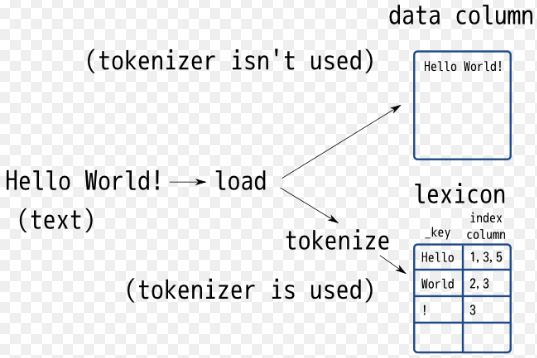
\includegraphics[width=1\textwidth]{figures/c7t/1.JPG}}
	\caption{Tokenizer}
	\label{c7t_1}
\end{figure}
\item Penjelasan mengenai Deep Learning.
\subitem Deep Learning adalah salah satu cabang dari Machine Learning atau dapat dikatakan bagian keluarga yang lebih luas dari method machine learning berdasarkan pada representasi data pembelajaran dan memiliki konsep serupa, tapi dilakukan dengan metode yang lebih cerdas. Deep Learning menggunakan Deep Neural Network dalam melakukan suatu penyelesaian suatu masalah yang terjadi pada Machine Learning.
\item Penjelasan apa itu Deep Neural dan bedanya dengan Deep Learning.
\begin{itemize}
\item Deep Neural Network atau DNN adalah sebuah algoritma yang berbasis neural network yang bisa digunakan untuk mengambil sebuah keputusan.
\item Dan yang membedakan Deep Learning dengan Deep Neural Network (DNN) adalah DNN merupakan algoritma yang digunakan pada Deep Learning, sedangkan Deep Learning merupakan model yang menggunakan algoritma DNN.
\end{itemize}
\end{enumerate}